\makeatletter
\def\input@path{{../../}}
\makeatother
\documentclass[../../main.tex]{subfiles}

\graphicspath{
	{../../img/}
	{../img/}
	{img/}
}

\begin{document}

\begin{proof}
	Полагая
	\[ u = u(x, y) = \Re f(z), \]
	\[ v = v(x, y) = \Im f(z), \]
	имеем
	\begin{equation}
		\label{lec31:1}
		 I = \oint\limits_{l} f(z) dz \stk{lec30_2:5}=
		\underbrace{ \oint\limits_{l} u dx - v dy }_{I_1}
		\ + \ i \underbrace{ \oint\limits_{l} v dx + u dy }_{I_2}
	\end{equation}
	Из непрерывной дифференцируемости $f(z)$ следует непрерывная
	дифференцируемость действительных Ф2П $u = u(x, y)$ и $ v = v(x, y)$.
	Воспользуемся условиями Коши-Римана для обоснования того факта, что в
	\eqref{lec31:1} $I_1 = I_2 = 0$. Для этого воспользуемся условиями
	Эйлера независимости КрИ-2 от пути интегрирования
	($P'_y = Q'_x$):
	\begin{enumerate}
		\item $\begin{cases}
				P = u \\
				Q = -v
			\end{cases} \hspace{-1em} \implies P'_y = u'_y = -v'_x = Q'_x
			\implies I_1 = 0,$
		\item $\begin{cases}
			P = v \\
			Q = u
		\end{cases} \hspace{-1em} \implies P'_y = v'_y = u'_x = Q'_x
		\implies I_2 = 0$.
	\end{enumerate}
	Следовательно, $I = 0$.
\end{proof}
\begin{rems}
	\
\begin{enumerate}
		\item Можно показать, что теорема выполняется и на менее сильных
			условиях на $f(z)$. Достаточна лишь дифференцируемость $f(z)$,
			но при этом доказательство сильно усложняется.
		\item Если $f(z)$ аналитична в $D$, т.~е. дифференцируема в каждой
			точке $D$ и непрерывна в замыкании $D = \partial D \cup D$,
			то тогда в случае, когда граница $ l = \partial D$ является
			кусочно-гладким контуром, доказанная теорема верна и для
			контура
			\[ \oint\limits_{\partial D} f(z) dz = 0. \]
		\item Теорема естественным образом обобщается на случай
			многосвязной области $D$, при этом под границей $l$
			подразумевается ее полная граница, например:
			\[ l = l_1^+ \cup l_2^- \cup l_3^-.\]
			\begin{center}
			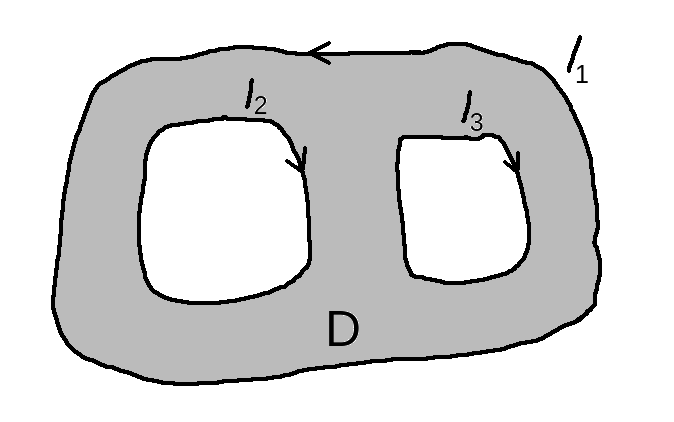
\includegraphics[scale = 0.3]{lec31_1.png}
			\end{center}
\end{enumerate}
\end{rems}

Идея доказательства для двусвязной области следующая:
\begin{center}
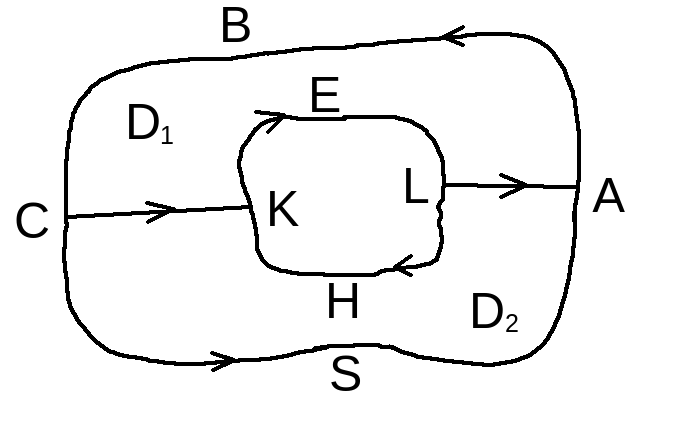
\includegraphics[scale = 0.3]{lec31_2.png}
\end{center}
\[ \partial D_1 = \overrightarrow{CK} \cup \overrightarrow{KEL}
\cup \overrightarrow{LA} \cup \overrightarrow{ABC} \]
\[ \partial D_2 = \overrightarrow{CSA} \cup \overrightarrow{AL} \cup
\overrightarrow{LHK} \cup \overrightarrow{KC} \]
Имеем
\[ \int\limits_{\overrightarrow{CK}} +
\int\limits_{\overrightarrow{KC}} = 0, \qquad\qquad
\int\limits_{\overrightarrow{LA}} +
\int\limits_{\overrightarrow{AL}} = 0, \qquad\qquad
\oint\limits_{\partial D_1} = 0, \qquad\qquad
\oint\limits_{\partial D_2} = 0, \]
откуда
\[ \oint\limits_{\partial D_1 \cup \partial D_2} = 
\oint\limits_{\partial D_1} + \oint\limits_{\partial D_2} = 0 \implies\]
\[\implies
\left( \oint\limits_{\overrightarrow{CK}} + 
\oint\limits_{\overrightarrow{KEL}} +
\oint\limits_{\overrightarrow{LA}} +
\oint\limits_{\overrightarrow{ABC}} \right) + \left(
\oint\limits_{\overrightarrow{CSA}} +
\oint\limits_{\overrightarrow{AL}} +
\oint\limits_{\overrightarrow{LHK}} +
\oint\limits_{\overrightarrow{KC}} \right)
= \oint\limits_{\overrightarrow{ABCSA}} +
\oint\limits_{\overrightarrow{KELHK}} = 0. \]
\begin{crl*}[независимость интеграла аналитической ФКП от пути
	интегрирования]
	Если $f(x)$ аналитична на $D$, то для $ \forall z_1, z_2 \in \C $
	и для любых кусочно-гладких путей $ l_1, l_2 \in D$, соединяющих
	$ z_1 $ и $ z_2 $ выполняется
	\[ \int\limits_{l_1} f(z) dz =
	\int\limits_{l_2} f(z) dz. \]
\end{crl*}
\begin{proof}
Рассмотрим замкнутый путь $ l = l_1^+ \cup
l_2^- $:
\begin{center}
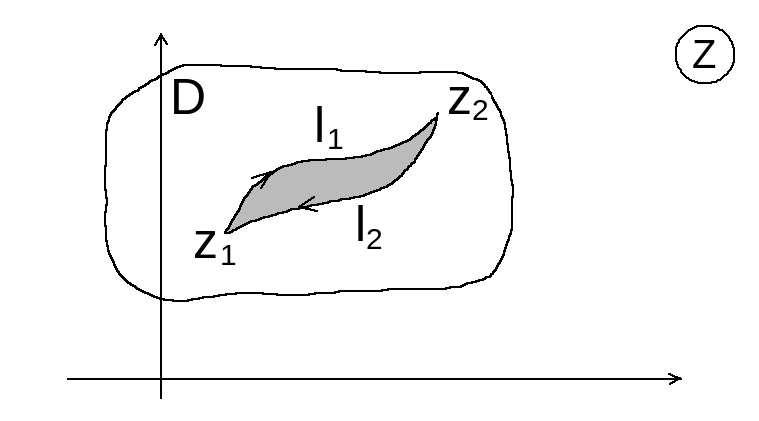
\includegraphics[scale = 0.3]{lec31_3.png} 
\end{center}
С учетом доказанной далее теоремы, из аналитичности $f(z)$ следует ее
бесконечная непрерывная дифференцируемость. Тогда 
\[ 0 = \int\limits_{l} f(z) dz = \int\limits_{l_1^+} f(z) dz +
\int\limits_{l_2^-} f(z) dz 
 \implies \int\limits_{l_1^+} f(z) dz =
- \int\limits_{l_2^-} f(z) dz = \int\limits_{l_2^+} f(z) dz.\qedhere\]
\end{proof}
\section{Первообразная аналитической ФКП}
Для ФКП $ f(z),\ z \in D \subset \C $ дифференцируемую функцию $F(z),\ z \in
D$ будем называть \emph{первообразной} для $f(z)$, если 
\begin{equation}
	\label{lec31:2}
	\forall z \in D \quad \exists F'(z) = f(z).
\end{equation}
\begin{thm}[о первообразной для аналитической ФКП]
	Для аналитической в односвязной области $D$ ФКП $f(z)$ существует хотя бы
	одна первообразная $F(z),\ z \in D$, и в качестве одной из первообразных
	можно взять интеграл с переменным верхним пределом
	\begin{equation}
		\label{lec31:3}
		\Phi(z) = \int\limits_{\scriptsize\overbowright{z_0 z}} f(t) dt =
		\int\limits_{z_0}^z f(t) dt, \quad \forall z \in D, \ l =
		\overbowright{z_0 z} \subset D.
	\end{equation} 
\end{thm}
\begin{proof}
	Во первых, в силу независимости интеграла аналитической ФКП от пути
	интегрирования в односвязной области $D$, \eqref{lec31:3} корректно
	определена для $\forall z \in D$, т.~к. значение интеграла в
	\eqref{lec31:3} не зависит от пути $l \subset D$, соединяющего $z_0$
	и $z$. Для $\forall z \in D$, придавая произвольное приращение $\Delta z \in 
	\C$ так, чтобы $z + \Delta z
	\in D$, имеем:
	\begin{equation}
		\label{lec31:4}
		\Delta \Phi(z) = \Phi(z + \Delta z) - \Phi(z) =
		\int\limits_{z_0}^{z + \Delta z} f(t) dt - 
		\int\limits_{z_0}^{z} f(t) dt =
		\int\limits_{z}^{z + \Delta z} f(t) dt.
	\end{equation}
	\begin{center}
	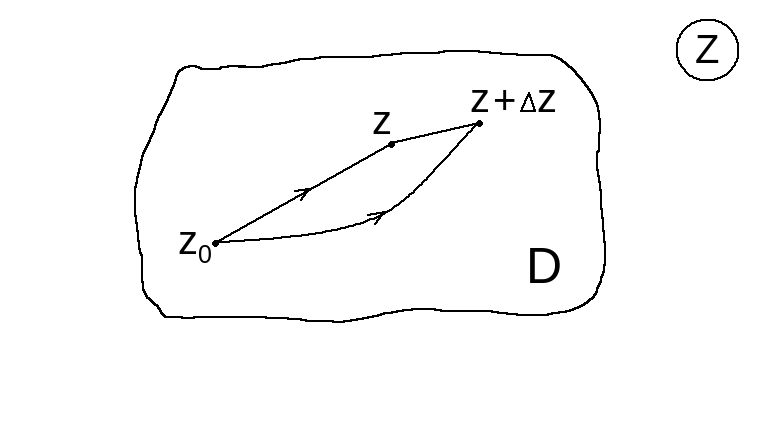
\includegraphics[scale = 0.3]{lec31_4.png}
	\end{center}
	Отсюда для $ \Delta z \neq 0$ получаем:
	\begin{equation}
	\begin{gathered}
		\label{lec31:5}
		\left| \dfrac{\Delta \Phi(z)}{\Delta z} - f(z) \right|
		\stackrel{ \eqref{lec31:4} }{=} \left|
		\dfrac{1}{\Delta z} \int\limits_{z}^{z + \Delta z} f(t) dt - f(z)
		\right| = \left|
		\dfrac{1}{\Delta z} \int\limits_{z}^{z + \Delta z} f(t) dt - 
		\dfrac{f(z)}{\Delta z} \int\limits_{z}^{z + \Delta z} dt
		\right| = \\
		= \left| \dfrac{1}{\Delta z} \int\limits_{z}^{z + \Delta z}
		(f(t) - f(z) ) dt \right| \le
		\dfrac{1}{ | \Delta z | } \left| \int\limits_{z}^{z + \Delta z}
		| f(t) - f(z) | | dt | \right|.
	\end{gathered}	
	\end{equation}
	Далее, в силу того что $D$ --- односвязное множество, мы можем заключить 
	путь
	$ l_0 = \overbowright{z, \ z + \Delta z} \subset D$ в 
	некоторый компакт $ l_0 \subseteq D_0 \subset D$. В результате
	непрерывная $f(z)$ на компакте $D_0 \subset D$ будет равномерно
	непрерывной на $D_0$, а значит, и на $l_0$, поэтому
	\[ \forall \eps > 0 \quad \exists \delta = \delta_\eps
	> 0 \quad \forall z, t \in l_0 \quad |z - t| \leq \delta
	\implies |f(z) - f(t)| \leq \eps. \]
	В результате, используя вместо $t$ величину $ z + \Delta z $, получаем, что
	если $| \Delta z| \le \delta$, то
	${| f(z + \Delta z ) - f(z) | \leq \eps}$.
	Поэтому
	\[ \left| \dfrac{\Delta \Phi(z)}{\Delta z} - f(z) \right|
	\stackrel{ \eqref{lec31:5} }{\le}
	\dfrac{1}{ | \Delta z | } \left| \int\limits_{z}^{z + \Delta z}
	\eps dt \right| = 
	\dfrac{\eps}{ | \Delta z | } \left| z + \Delta
	z - z \right| = \eps.\]
	Поэтому
	\[ \exists \Phi ' (z) = \lim\limits_{\Delta z \to 0}
	\dfrac{\Delta \Phi(z)}{\Delta z} = f(z). \]	
	\eqref{lec31:3} будет одной из первообразных для $f(z)$.
\end{proof}

\begin{crl*}[общий вид первообразной для аналитичной ФКП]
	Для $ f(z) $ в $D$ любая ее первообразная $F(z)$ отличается от
	\eqref{lec31:3} на некоторую константу,
	т.~е.
	\begin{equation}
	\label{lec31:6}
		F(z) = \Phi(z) + c_0,\ c_0 = const \in \C.
	\end{equation}
\end{crl*}

\begin{proof}
Доказательство основано на:
\begin{thm}[критерий постоянства аналитической ФКП]
	Аналитическая $H(z)$ в односвязной области $D$ будет постоянной
	$\iff \forall z \in D \quad H'(z) = 0$.
\end{thm}
\begin{proof} ~

\nec:
Если $H(z) = const$, то $H'(z) = 0, \ \forall z \in D$.

\suff:
Пусть $H'(z) = 0, \ \forall z \in D$. Тогда для $\begin{cases}
	u = \Re H(z) \\
	v = \Im H(z)
\end{cases}$ \hspace{-1em} получаем \[H'(z) = u'_x + i v'_x = 0 \implies
u'_x \equiv 0, \ v'_x \equiv 0.\] Кроме того, в силу условия Коши-Римана:
\[ u'_y = -v'_x = 0, \]
\[ v'_y = u'_x = 0.\]
Значит, $\begin{cases} v'_x \equiv 0 \\ v'_y \equiv 0
\end{cases} \hspace{-1em} \implies v $ не зависит от $x$ и $y$, откуда 
следует, что $ v(x, y) = const = c_1 $.
Аналогично $\begin{cases} u'_x \equiv 0 \\ u'_y \equiv 0
\end{cases} \hspace{-1em} \implies u = const = c_2 $.
Тогда $H(z) = u + i v = c_2 + i c_1 = c \in \C $.
\end{proof}

Применяя этот критерий к функции \[ H(z) = F(z) - \Phi(z) = F(z) -
\int\limits_{z_0}^z f(t) dt,\] получаем, что $ H'(z) = F'(z) - \Phi ' (z) =
f(z) - f(z) = 0$, если $F(z)$ --- одна из первообразных для $f(z)$.
Значит, $H(z) \equiv const = c_0 \in \C \implies F(z) = \Phi(z) + c_0$.
\end{proof}

\begin{rem}[аналог формулы двойной подстановки для интеграла ФКП]
	Если $f(z)$ аналитична в односвязной области $D$, а $F(z)$ --- её
	первообразная, то
	\begin{equation}
		\label{lec31:7}
		\forall z_1, z_2 \in D \implies \int\limits_{z_1}^{z_2} f(t) dt =
		F(z_2) - F(z_1) = \left[ F(z) \right]_{z_1}^{z_2}.
	\end{equation}
\end{rem}
\begin{proof}
	Используя аддитивность интеграла ФКП, для $z_0 \in D$ имеем:
	\[ \int\limits_{z_1}^{z_2} f(z) dz =
	\int\limits_{z_1}^{z_0} f(t) dt + \int\limits_{z_0}^{z_2} f(t) dt =
	\int\limits_{z_0}^{z_2} f(t) dt - \int\limits_{z_0}^{z_1} f(t) dt
	\stackrel{ \eqref{lec31:3} }{=} \Phi(z_2) - \Phi(z_1)
	\stackrel{ \eqref{lec31:6} }{=}
	\] \[
	\stackrel{ \eqref{lec31:6} }{=} (F(z_2) - c_0) - (F(z_1) - c_0) =
	F(z_2) - F(z_1) = \left[ F(z) \right]_{z_1}^{z_2}. \qedhere
	\]
\end{proof}
\begin{crl*}[интегрирование по частям ФКП]
	Если $f(z), g(z)$ аналитичны в $D$, то для $\forall z_1, z_2 \in D$ 
	выполняется
\begin{equation}
	\label{lec31:8}
	\begin{gathered}
	\int\limits_{z_1}^{z_2} f(z) g'(z) dz = 
	\int\limits_{z_1}^{z_2} f(z) d(g(z)) =
	[f(z)g(z)]_{z_1}^{z_2} - \int\limits_{z_1}^{z_2} g'(z) d(f(z)) = \\ =
	f(z_2)g(z_2) - f(z_1)g(z_1) - \int\limits_{z_1}^{z_2} f'(z) g(z) dz.
	\end{gathered}
\end{equation}
\end{crl*}
\begin{example}
	\[I =  \int\limits_{[0, \pi + \pi i]} z \cos z\;dz. \]
	\begin{center}
	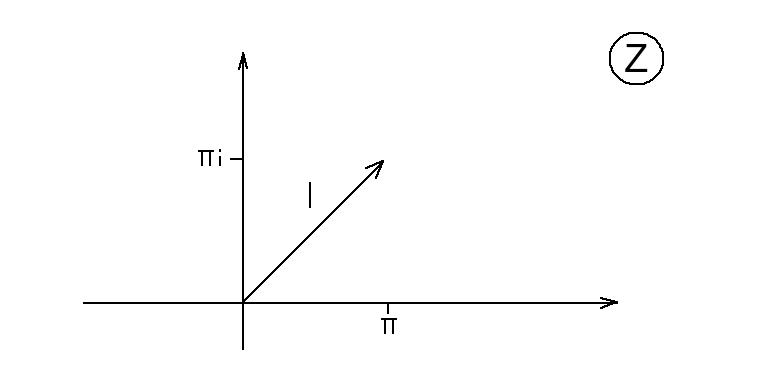
\includegraphics[scale = 0.3]{lec31_5.png}
	\end{center}
	$ f(z) = z \cos z $ аналитична в $\C$, следовательно, интеграл не
	зависит от пути интегрирования и можно воспользоваться
	интегрированием по частям:
	\[\begin{gathered}	
	z_1 = 0 \\
	z_2 = \pi + \pi i \end{gathered}\]
	\[\begin{gathered}
	I = \int\limits_{0}^{\pi + \pi i} z d(\sin z) =
	z \sin z |_0^{\pi + \pi i} -
	\int\limits_{0}^{\pi + \pi i} \sin z dz =
	(\pi + \pi i) \sin (\pi + \pi i) + [ \cos z ]_0^{\pi + \pi i} = \\ =
	(\pi + \pi i) ( - \sin \pi i) + \cos (\pi + \pi i) - 1 =
	(\pi + \pi i) \dfrac{\sh \pi}{i} - \cos \pi i - 1 = \\ =
	- \pi i \sh \pi + \pi \sh \pi - \ch \pi - 1.
	\end{gathered} \]
\end{example}
\end{document}
